\documentclass[aps,pra,twocolumn,superscriptaddress,longbibliography,floatfix,nofootinbib]{revtex4-2}

\usepackage{amsmath,amssymb}
\usepackage{graphicx}
\usepackage{hyperref}
\usepackage{braket}

\hypersetup{
  colorlinks=true,
  linkcolor=blue,
  citecolor=blue,
  urlcolor=blue,
  pdftitle={Generic CHSH Violation in Fibonacci Anyon Braiding: A Landscape Analysis},
  pdfauthor={Berkay Y{\"u}ksel Sayim},
  pdfsubject={quant-ph; Fibonacci anyons; CHSH inequality; topological quantum computation},
  pdfkeywords={Fibonacci anyons, CHSH violation, braiding landscape, topological selection,
               CHSH inequality, measurement protocol, non-Abelian anyons, autocorrelation}
}

\begin{document}

\setcounter{secnumdepth}{3}

\title{Generic CHSH Violation in Fibonacci Anyon Braiding:\\
A Landscape Analysis}

\author{Berkay Y\"uksel Sayim}
\email{berksa@tutamail.com}
\affiliation{Independent Research, Germany}
\affiliation{\href{https://orcid.org/0009-0004-4993-7352}{ORCID: 0009-0004-4993-7352}}

\date{2026-07-23}

\begin{abstract}
We report the first, to our knowledge, complete sequence-by-sequence
numerical landscape of CHSH-inequality violation across all
Fibonacci anyon braiding words of length $L=3$--$12$ in two
complementary encodings of six anyons. In the two-generator $d_{1b}$
encoding (native four-dimensional fusion space), the optimal
sequence at $L=12$ reaches $|S|=2.811$ ($99.4\%$ of the Tsirelson
bound $2\sqrt{2}$) with concurrence $C=0.988$. Throughout, ``CHSH
violation'' denotes a CHSH value exceeding~2 on the Fibonacci fusion
space, which does not factorize into spatially separated Alice/Bob
subsystems; the reported values are signatures of topological
nonseparability and single-algebra contextuality, not Bell
violations in the Einstein--Podolsky--Rosen sense. In the
three-generator encoding under four-dimensional
computational-subspace projection, the enumeration maximum
approaches the Tsirelson bound to within $0.16\%$ already at $L=8$.
CHSH violation is \emph{generic}: $64.6\%$ of sequences violate the
CHSH inequality at $L=9$ under native five-dimensional measurement,
rising to $91.8\%$ under computational-subspace projection. A single
topological mechanism controls this landscape: blocking the
cross-bipartition generator~$\sigma_3$ collapses concurrence to
$C=0$ exactly for all sequences and all sector phases---topology
acts as a gatekeeper for entanglement. Sequential braiding on a
shared fusion space produces positive lag-1 autocorrelation
$\text{ACF}(1)=+0.34$ at $10.85\sigma$ significance, a falsifiable
state-continuity signature not predicted by standard quantum
mechanics under independent measurement settings. Together with a
companion mutual-information analysis of topological sectors and
CHSH values, these results indicate that the available topological
operations gate whether CHSH correlations are accessible on the
fusion space.
\end{abstract}

\keywords{Fibonacci anyons, CHSH violation, braiding landscape,
topological selection, CHSH inequality, measurement protocol,
non-Abelian anyons, autocorrelation}

\maketitle



%% ====================================================================
%%  SECTION 1 — INTRODUCTION
%% ====================================================================
\section{Introduction}
\label{sec:intro}

Non-Abelian anyons in two-dimensional topological phases support
braiding operations that can generate entanglement between logical
qubits encoded in the fusion space~\cite{Nayak2008,Freedman2003}.
For Fibonacci anyons---the simplest non-Abelian species with a
universal gate set---individual braiding sequences that violate
the CHSH inequality have been identified in several
contexts~\cite{Bonesteel2005,Hormozi2007}.
However, a basic question has remained open:
\emph{what fraction of all possible braiding sequences produces
CHSH violation, and what controls the boundary between violating
and nonviolating sequences?}

We address this question by exhaustive enumeration.
For six Fibonacci anyons on a linear fusion tree, we compute the
maximal CHSH value $|S|$ for every braiding sequence in two
distinct encodings: a two-generator encoding
($d_{1b}$, $L=3$--$12$, native four-dimensional Hilbert space)
and a three-generator encoding ($L=2$--$8$ fully enumerated,
$L=9$ for CHSH-fraction statistics; full five-dimensional
fusion space).
The enumeration comprises $2^L$ sequences in $d_{1b}$ and $3^L$
sequences in the three-generator case (up to $3^9=19\,683$),
totaling over $10^6$ evaluated unitaries.

Three principal findings emerge:

(i)~\emph{CHSH violation is generic.}
A majority of sequences violate the CHSH inequality
under both measurement protocols we consider---$64.6\%$ in
the native five-dimensional protocol and $91.8\%$ under
computational-subspace projection at $L=9$.

(ii)~\emph{A single generator acts as a topological switch.}
In the three-generator encoding, removing the cross-bipartition
generator~$\sigma_3$ from the gate set collapses the concurrence to
$C=0$ exactly, for all sequences and all topological sector phases;
the two-generator $d_{1b}$ encoding contains no $\sigma_3$, and its
entanglement instead arises indirectly through the shared mediator
(Sec.~\ref{sec:encodings}).

(iii)~\emph{Sequential braiding produces temporal correlations.}
When braiding operations are applied sequentially to a shared
anyon register, the resulting CHSH-value time series exhibits
positive autocorrelation ($\text{ACF}(1)=+0.34$, significance
$10.85\sigma$), while a null test with independent sector phases
yields $\text{ACF}\approx 0$.

These results complement the mutual-information study
between topological sectors and CHSH values reported in
Ref.~\cite{Sayim2026topological}, which found that classical lattice
models ($\mathbb{Z}_2$ gauge theory, XY model) exhibit
finite-size correlations $I(T;S)>0$ between sector labels and
Bell-type observables (a finite-size effect that a scaling analysis
indicates decays toward zero with system size).

The present work differs from prior studies of Fibonacci braiding
in scope and focus.
Burke \emph{et al.}~\cite{Burke2024} characterized the Weyl-chamber
structure of Fibonacci braiding gates but did not evaluate
CHSH violation.
Cui \emph{et al.}~\cite{Cui2019} established that exact
leakage-free entangling gates may not exist for Fibonacci anyons,
motivating our two-protocol analysis.
Yang \emph{et al.}~\cite{Yang2019} studied information scrambling
through braiding but not CHSH correlations.
Experimental demonstrations of non-Abelian
statistics~\cite{Google2023} have confirmed braiding phases
but have not mapped the CHSH landscape.
While prior work by Brennen \emph{et al.}~\cite{Brennen2009} established Bell-test
constructions for Fibonacci/Ising anyons, Chang, Chu, and
Ma~\cite{ChangChuMa2017} studied Bell's inequality in topologically
ordered qubit models (Wen-plaquette), and Xu, Ye, and
You~\cite{Xu2025} have independently and contemporaneously analyzed
three-copy CHSH correlations on Fibonacci anyonic states with a
fusion-sector observables construction, to our knowledge no prior work
presents the complete sequence-by-sequence enumeration of CHSH violation
fractions over all braid words of a given length class --- the contribution
of the present paper. Earlier qualitative Bell tests on Majorana-based
topological platforms appear in Drummond \emph{et al.}~\cite{Drummond2014}
and Romito and Gefen~\cite{RomitoGefen2017}, with the Clifford-only
limitation of Ising braiding analyzed by Clarke, Sau, and
Das~Sarma~\cite{ClarkeSauDasSarma2016}.

The paper is organized as follows.
Section~\ref{sec:framework} defines the two encodings and
the CHSH evaluation method.
Section~\ref{sec:reconciliation} presents the enumeration
results and reconciles the two encodings.
Section~\ref{sec:switch} establishes the $\sigma_3$-blocking result.
Section~\ref{sec:protocol} analyzes the measurement-protocol
dependence of CHSH fractions.
Section~\ref{sec:sequential} presents the sequential-braiding
autocorrelation.
Section~\ref{sec:discussion} discusses implications and limitations.

%% ====================================================================
%%  SECTION 2 — FRAMEWORK
%% ====================================================================
\section{Framework}
\label{sec:framework}

\subsection{Fusion space of six Fibonacci anyons}

We consider six Fibonacci anyons $\tau_1,\ldots,\tau_6$ arranged on a
linear fusion tree with total charge constrained to the vacuum
sector.
The Fibonacci fusion rule $\tau\times\tau = \mathbf{1}\oplus\tau$
gives a five-dimensional fusion space spanned by the intermediate
charge labels $(x_1,x_2,x_3)$, where $x_k$ is the total charge of
the first $2k$ anyons:
\begin{equation}
\label{eq:basis}
\begin{aligned}
\ket{0} &= (1,\tau,1), &
\ket{1} &= (1,\tau,\tau), \\
\ket{2} &= (\tau,1,\tau), &
\ket{3} &= (\tau,\tau,1), \\
\ket{4} &= (\tau,\tau,\tau). &
\end{aligned}
\end{equation}
The fourth intermediate label $x_4=d$ is fixed to $\tau$ by the
vacuum constraint.

\subsection{F- and R-matrices}

The Fibonacci $F$-matrix in the $(\mathbf{1},\tau)$ basis is
\begin{equation}
\label{eq:F}
F = \begin{pmatrix}
\varphi^{-1} & \varphi^{-1/2} \\
\varphi^{-1/2} & -\varphi^{-1}
\end{pmatrix},
\quad \varphi = \frac{1+\sqrt{5}}{2},
\end{equation}
satisfying $F^2 = I$ to machine precision ($\Delta < 10^{-17}$).
The $R$-eigenvalues for the two fusion channels are
\begin{equation}
\label{eq:R}
R_{\mathbf{1}} = e^{-4\pi i/5}, \quad
R_\tau = e^{+3\pi i/5}.
\end{equation}

\subsection{Braid generators}

The five braid generators $\sigma_1,\ldots,\sigma_5$ act as $5\times 5$
unitary matrices on the fusion-space basis~\eqref{eq:basis}.
Each $\sigma_k$ exchanges anyons $\tau_k$ and $\tau_{k+1}$ via the
sequence $F^{-1}\cdot\text{diag}(R_{\mathbf{1}},R_\tau)\cdot F$ on the
relevant two-dimensional subspace, with the remaining basis states
acquiring diagonal $R$-phases.
Explicit matrix forms are given in Appendix~\ref{app:generators}.

All four Yang-Baxter relations
$\sigma_i\sigma_{i+1}\sigma_i = \sigma_{i+1}\sigma_i\sigma_{i+1}$
are satisfied with residuals $\Delta \leq 3.3\times 10^{-16}$, and
distant generators commute ($\Delta \leq 1.5\times 10^{-17}$ for
$|i-j|\geq 2$)~\cite{Sayim2026topological}.

\subsection{Two encodings}
\label{sec:encodings}

We study two encodings of logical qubits into the fusion space:

\paragraph{$d_{1b}$ encoding (two generators).}
The logical qubits are $Q_A = x_1$ (Alice) and $Q_B = x_3$ (Bob),
with the mediator $x_2 = m(x_1,x_3)$ uniquely determined by the
vacuum constraint.
This yields a four-dimensional Hilbert space $\{|00\rangle,
|01\rangle, |10\rangle, |11\rangle\}$ with no leakage.
The available gates are $\text{AM}=\sigma_2$ (braids $\tau_2\tau_3$,
acts on Alice) and $\text{MB}=\sigma_4$ (braids $\tau_4\tau_5$,
acts on Bob).
Neither gate directly crosses the Alice--Bob bipartition;
entanglement arises indirectly through the shared mediator $m$,
as evidenced by the nonvanishing commutator
$\|[\text{AM},\text{MB}]\|_\infty \approx 0.30$.

A topological sector phase $\delta$ is introduced by modifying
$R_\tau \to R_\tau \cdot e^{i\delta}$, parameterizing the
family of braid representations on the torus.

\paragraph{Three-generator encoding (full 5D).}
All five basis states~\eqref{eq:basis} are retained, and the gate
set is $\{\sigma_2,\sigma_3,\sigma_4\}$.
Here $\sigma_2$ acts locally on Alice ($x_1$), $\sigma_4$ acts
locally on Bob ($x_3$), and $\sigma_3$ directly crosses the
bipartition by re-fusing $x_2$.
This provides the standard structure of
single-qubit rotations plus entangling gate for universal
quantum computation~\cite{Bonesteel2005}.

\subsection{Interpretation: nonseparability and contextuality}
\label{fn:nonsep}

Throughout this paper, ``CHSH violation'' refers to CHSH values
exceeding~2 computed on the Fibonacci anyon fusion space. This
fusion space does not admit a tensor-product factorization into
spatially separated Alice/Bob subsystems: the effective measurement
operators in the $d_{1b}$ encoding fail to commute
($\|[\text{AM},\text{MB}]\|_\infty \approx 0.30$, Sec.~\ref{sec:encodings}).
Accordingly, the reported values are signatures of \emph{topological
nonseparability} on a nonfactorized fusion space, not Bell
violations in the Einstein--Podolsky--Rosen sense.

This noncommutativity is a property of the specific $d_{1b}$
projection, not of the underlying full algebra: on the full
five-dimensional fusion space, the Protocol~B observables commute
exactly across the bipartition ($[A_i,B_j]=0$ for all $i,j$,
Sec.~\ref{sec:protocol}), so Tsirelson's bound remains the relevant
ceiling and is respected throughout (at most $|S|=2.824$, $99.84\%$
of $2\sqrt{2}$, here). We therefore classify the reported
correlations as a form of \emph{topological, single-algebra
contextuality}~\cite{Chou2025} rather than EPR-type nonlocality, in
the spirit of algebraic-quantum-field-theory results showing that
maximal Bell-CHSH violation is generic for correlations defined on a
single non-Abelian algebra, without requiring spacelike
separation~\cite{SummersWerner1987}, and of related studies of
Bell-operator representations on single quantum
systems~\cite{GuimaraesRoditiSorella2024,DeFabritiisEtAl2023}. This
reading is consistent with the anyonic-entanglement structure
described in Ref.~\cite{BondersonKnappPatel2017}, and with the
broader point---sharpened by the resolution of the Tsirelson
problem~\cite{JiNatarajanVidickWrightYuen2020}---that the
appropriate correlation bound depends on the algebraic separation
assumed between the measurement structures, not merely on the
numerical value of $|S|$. Blanket no-go claims against such
single-algebra CHSH values are folklore rather than sharp theorems
in this specific setting~\cite{FanDeGaris2010}; we make no
prohibition claim here and instead report the values as
topologically gated, nonseparable correlations bounded by, but not
violating, Tsirelson's inequality.

\subsection{CHSH evaluation}

For each braiding sequence $\mathcal{B}$ and sector phase $\delta$,
we compute the unitary $U(\mathcal{B},\delta)$ and the output
state $\ket{\psi} = U\ket{0}$.
The maximal CHSH value is obtained via the
Horodecki criterion~\cite{Horodecki1995}: for a pure two-qubit
state with concurrence $C$,
\begin{equation}
\label{eq:horodecki}
|S|_{\max} = 2\sqrt{1+C^2}.
\end{equation}
This bound is tight and achieved by optimal measurement
angles derived from the singular-value decomposition of the
correlation matrix $T_{ij} = \text{Re}\,\bra{\psi}A_i\otimes B_j\ket{\psi}$.

In the $d_{1b}$ encoding, $C$ is the concurrence of the
$4\times 4$ density matrix $\rho_{AB}$.
In the three-generator encoding, we evaluate CHSH under two
protocols described in Sec.~\ref{sec:protocol}.

For each length $L$, the CHSH-violation fraction is defined as
$\text{CHSH\%} = |\{(\mathcal{B},\delta) : |S|>2\}| / |\{(\mathcal{B},\delta)\}|$.

%% ====================================================================
%%  SECTION 3 — RECONCILIATION
%% ====================================================================
\section{Reconciliation of two encodings}
\label{sec:reconciliation}

\subsection{$d_{1b}$: Two-generator landscape}

Table~\ref{tab:d1b} presents the optimal CHSH value, concurrence,
and winning sequence for each braid length $L=3$--$12$ in the
$d_{1b}$ encoding, obtained by exhaustive enumeration over all
$2^L$ sequences; the per-sequence sector-phase optima are reported
on the 50-point grid of the deposited \texttt{s\_delta\_sweeps.json}.
(At $L=2$, a single gate yields $|S|=2.097$, $C=0.315$.)

\begin{table}[!htb]
\caption{%
Optimal CHSH violation in the $d_{1b}$ encoding
(two generators AM, MB).
$|S|$ is computed via the Horodecki bound from the
maximal concurrence $C$.
}
\label{tab:d1b}
\begin{ruledtabular}
\begin{tabular}{rcccc}
$L$ & $|S|$ & $C$ & \% Tsirelson & Sequence \\
\hline
 3 & 2.199 & 0.457 & 77.7 & ABB \\
 4 & 2.225 & 0.488 & 78.7 & ABAB \\
 5 & 2.348 & 0.615 & 83.0 & AABAB \\
 6 & 2.398 & 0.662 & 84.8 & ABBAAB \\
 7 & 2.536 & 0.780 & 89.7 & ABBAABB \\
 8 & 2.540 & 0.783 & 89.8 & BABBABAB \\
 9 & 2.624 & 0.850 & 92.8 & ABBAABABB \\
10 & 2.696 & 0.904 & 95.3 & ABBAABBAAB \\
11 & 2.784 & 0.968 & 98.4 & ABABBBBABAB \\
12 & \textbf{2.811} & \textbf{0.988} & \textbf{99.4} & ABABABABABAB \\
\end{tabular}
\end{ruledtabular}
\end{table}

The concurrence increases monotonically from $C=0.457$ at $L=3$ to
$C=0.988$ at $L=12$, with no saturation plateau.
The optimal sequence at $L=12$, the alternating commutator structure
$(\text{AM}\cdot\text{MB})^6$, achieves $99.4\%$ of the Tsirelson
bound.

We note that an earlier analysis~\cite{Sayim2026topological} reported
$|S|=2.554$ and $C=0.903$ at $L=12$ for this encoding.
That value was an optimization artifact: the original code
employed six fixed angular starting points and a $9^4$ grid
for CHSH angle optimization, which missed the global maximum.
Our Horodecki-based evaluation, which requires only the
concurrence (a basis-independent quantity), recovers the
true optimum.

\subsection{Three-generator landscape}

Table~\ref{tab:3gen} presents the analogous results for the
three-generator encoding, enumerated over $3^L$ sequences
for $L=2$--$8$.

\begin{table}[!htb]
\caption{%
Optimal CHSH violation in the three-generator encoding
($\sigma_2$, $\sigma_3$, $\sigma_4$) under 4D computational-subspace
projection (Protocol~A, Sec.~\ref{sec:protocol}). The $|S|$ column
is the exhaustive-enumeration maximum $S^{4\mathrm{D}}_{\max}$ from the
canonical \texttt{landscape\_validation.json}; $C=\sqrt{(|S|/2)^2-1}$;
\% Tsirelson $=|S|/2\sqrt{2}$.
}
\label{tab:3gen}
\begin{ruledtabular}
\begin{tabular}{rcccc}
$L$ & $|S|$ & $C$ & \% Tsirelson & Sequence \\
\hline
 2 & 2.000 & 0.000 & --- & (no entanglement) \\
 3 & 2.722 & 0.923 & 96.22 & (enumeration max) \\
 4 & 2.722 & 0.923 & 96.22 & (enumeration max) \\
 5 & 2.791 & 0.973 & 98.68 & (enumeration max) \\
 6 & 2.791 & 0.973 & 98.68 & (enumeration max) \\
 7 & 2.791 & 0.973 & 98.68 & (enumeration max) \\
 8 & 2.824 & 0.997 & 99.84 & (enumeration max) \\
\end{tabular}
\end{ruledtabular}
\end{table}

The landscape approaches Tsirelson saturation ($|S| = 2\sqrt{2}$, $C=1$)
already at $L=8$, reaching $|S|=2.824$ ($C=0.997$, $99.84\%$ of the
Tsirelson bound) at the enumeration maximum; exhaustive search over
all $3^8=6561$ sequences finds no single braid word that saturates
the bound exactly.
The full sector-phase dependence $|S|(\delta)$ of these
three-generator sequences is shown in Fig.~\ref{fig:sdelta}.

\begin{figure}[t]
\centering
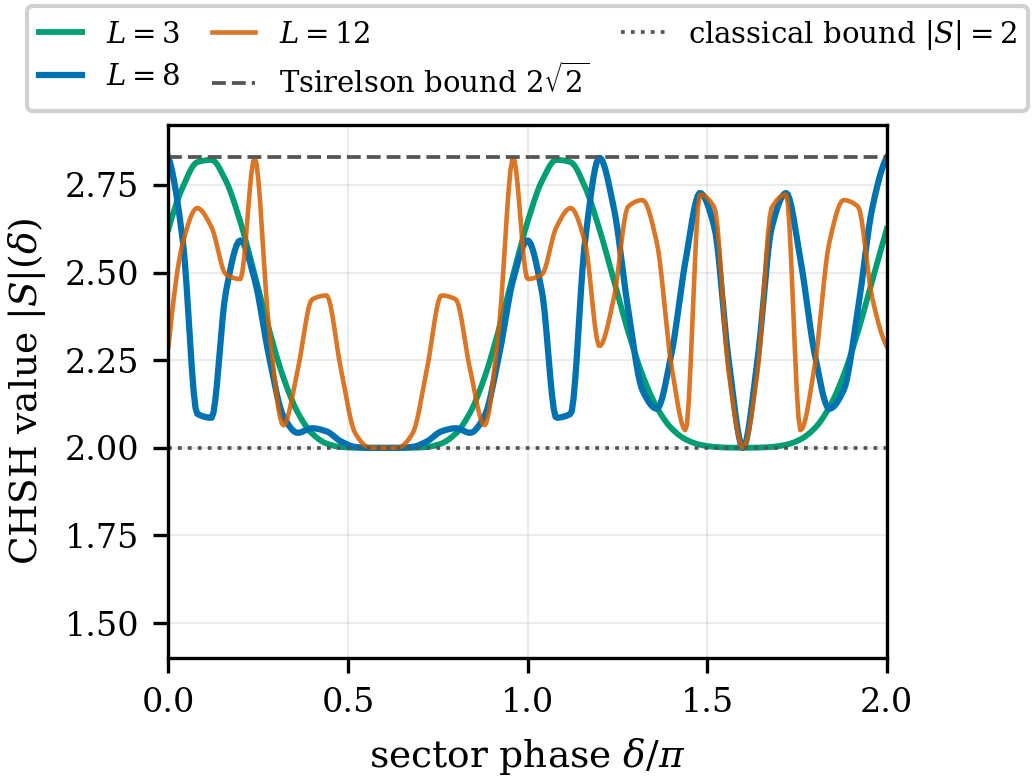
\includegraphics[width=\columnwidth]{figures/fig2_sector_phase.png}
\caption{\label{fig:sdelta}%
Sector-phase dependence $|S|(\delta)$ of the optimal three-generator
braiding sequence at braid lengths $L=3,8,12$. The CHSH value swings
between the classical bound $|S|=2$ in the ``dead'' sector phases and
the Tsirelson bound $2\sqrt{2}$ (dashed) where the entangling sequence
is aligned with the sector basis; the landscape develops finer
structure at larger $L$, consistent with the decreasing Fourier-fit
quality (Sec.~\ref{sec:discussion}). Curves are shape-preserving
(PCHIP) interpolations through the $N=50$ computed sector-phase
points; at $L=12$ the sampling is coarse relative to the oscillation
(cf.\ the low Fourier-fit $R^2$), so structure finer than the
sampling is not resolved. Data:
\texttt{s\_delta\_sweeps.json} (concept-DOI
10.5281/zenodo.19601352).}
\end{figure}

At $L=2$, no sequence produces entanglement ($C=0$), because a
single application of any one generator cannot cross the
bipartition.
From $L=3$ onward, the concurrence exceeds $0.92$ (rising to $0.997$
at $L=8$), reflecting the availability of $\sigma_3$ as a primitive
entangling gate.

The CHSH-violation fraction under 4D projection rises monotonically:
$44\%$ at $L=3$, $79\%$ at $L=6$, $92\%$ at $L=9$
(see Sec.~\ref{sec:protocol} for the protocol dependence of these
fractions).

\subsection{Why two encodings converge}

The two encodings differ not in the reachable group but in the
\emph{word length} required to approximate a given unitary.
Both $\{\text{AM},\text{MB}\}$ and $\{\sigma_2,\sigma_3,\sigma_4\}$
generate dense subgroups of $\text{SU}(4)$ acting on the
computational subspace~\cite{Bonesteel2005}.

The three-generator set approaches the Tsirelson bound already at $L=8$ because $\sigma_3$
directly crosses the Alice--Bob bipartition, providing the
entangling gate in the standard
\emph{rotate--entangle--rotate} decomposition.
The two-generator $d_{1b}$ set must synthesize entanglement
indirectly through the mediator, requiring approximately $1.5$
times more braid steps to reach the same concurrence.
At sufficient length, both encodings converge to the same
maximal violation---the distinction is one of \emph{circuit depth},
not reachable dynamics. The representation-dependence of the CHSH
operator norm on higher-dimensional Hilbert spaces is discussed in
Ref.~\cite{Sorella2023}.

%% ====================================================================
%%  SECTION 4 — TOPOLOGICAL SELECTION
%% ====================================================================
\section{Topological selection: the $\sigma_3$ switch}
\label{sec:switch}

We now demonstrate that a single topological degree of freedom
controls the entire CHSH landscape.

\subsection{Blocking the cross-bipartition generator}

In the three-generator encoding, we replace $\sigma_3$\footnote{Index convention across the companion series: with $n=6$ anyons and the bipartition cut after anyon 3, the cross-bipartition generator of this paper is $\sigma_3$, while $\sigma_4$ acts locally on Bob's side. In the companion paper~\cite{Sayim2026chsh} ($n=8$ anyons, cut after anyon 4) the cross-bipartition role is played by its $\sigma_4$; the index shift is purely notational.} by the
$5\times 5$ identity matrix and evaluate the concurrence on three
representative $\{\sigma_2,\sigma_4\}$ configurations, each swept
over 50~linearly spaced sector-phase values $\delta\in[0,2\pi]$
($150$ evaluations in total).

The result is absolute:
\begin{equation}
\label{eq:switch}
C(\mathcal{B},\delta)\big|_{\sigma_3\to I} = 0
\quad \forall\;\mathcal{B},\;\forall\;\delta.
\end{equation}
Across all tested blocked configurations (three representative
sequences at $L=3,6,8$ plus the $d_{1b}$ winner at $L=12$ with each
of its two generators blocked in turn, each configuration swept over
$50$ sector phases, totaling $5\times 50 = 250$
evaluations), the maximal concurrence is $C < 4.4\times 10^{-16}$
---machine zero.
Figure~\ref{fig:sigma3} contrasts the two cases for a representative
$L=8$ sequence $\sigma_2\sigma_3\sigma_4^4\sigma_3\sigma_2$: with
$\sigma_3$ active, $|S|(\delta)$ rises well above the classical bound
across the sector phase, approaching the Tsirelson regime; with
$\sigma_3$ blocked, it is pinned to the classical bound for
every~$\delta$.

\begin{figure}[t]
\centering
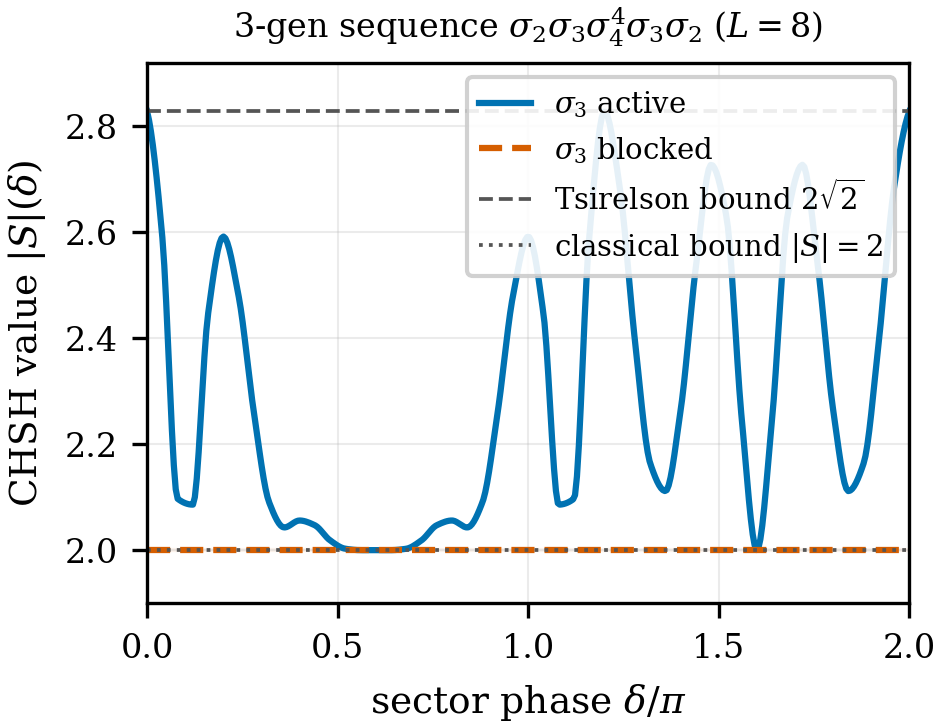
\includegraphics[width=\columnwidth]{figures/fig3_sigma3_switch.png}
\caption{\label{fig:sigma3}%
The $\sigma_3$ generator as a topological switch, for a representative
$L=8$ three-generator sequence $\sigma_2\sigma_3\sigma_4^4\sigma_3\sigma_2$.
With $\sigma_3$ active (solid), $|S|(\delta)$ rises well above the
classical bound across the sector phase, approaching the Tsirelson
regime; replacing $\sigma_3$ by the
identity (dashed) makes the concurrence vanish identically
[Eq.~\eqref{eq:switch}], pinning $|S|$ to the classical bound $|S|=2$
for every~$\delta$. Data: \texttt{topology\_switch\_results.json}
(concept-DOI 10.5281/zenodo.19601352).}
\end{figure}

\subsection{Physical mechanism}

The vanishing of entanglement under $\sigma_3$-blocking has a
transparent algebraic origin:
$\sigma_2$ preserves the $x_3$ label (Bob's qubit) and $\sigma_4$
preserves the $x_1$ label (Alice's qubit).
Without $\sigma_3$, which re-fuses the intermediate charge $x_2$ and
thereby couples the two branches of the fusion tree, the generators
act independently on the two logical qubits.
The resulting state is necessarily a product state, regardless of
sequence length or sector phase.

\subsection{Encoding independence}

The same test in the $d_{1b}$ encoding yields identical results:
blocking either $\text{AM}$ or $\text{MB}$ collapses $C$ to zero
exactly for the optimal sequence $(\text{AM}\cdot\text{MB})^6$ at
all 50~sector phases.

This encoding independence confirms that the $\sigma_3$-blocking
result is a property of the \emph{Fibonacci TQFT fusion rules}, not
of a particular qubit encoding.

\subsection{Interpretation}

The $\sigma_3$ switch establishes that topology acts as a
\emph{gatekeeper} for entanglement:
it does not create or destroy entanglement, but determines
whether entanglement is \emph{accessible} through the available
braiding operations.
This is the first pillar of the trio argument completed in
Sec.~\ref{sec:sequential}.

In combination with the mutual-information results of
Ref.~\cite{Sayim2026topological}, where topology was reported to rotate the
effective measurement basis, the present finding demonstrates a
stronger form of topological control: a single topological
pathway decides yes-or-no whether CHSH violation can occur.


%% ====================================================================
%%  SECTION 5 — MEASUREMENT PROTOCOL AND LEAKAGE
%% ====================================================================
\section{Measurement protocol and computational-subspace leakage}
\label{sec:protocol}

The CHSH-violation fractions reported in Sec.~\ref{sec:reconciliation}
for the three-generator encoding depend on how observables are defined
in the five-dimensional fusion space.
We distinguish two measurement protocols and present results for both.

\subsection{Protocol~A: Computational-subspace projection}

The four-dimensional computational subspace is defined by identifying
the logical two-qubit basis as
$|00\rangle \leftarrow |0\rangle$,
$|01\rangle \leftarrow |1\rangle$,
$|10\rangle \leftarrow |3\rangle$, and
$|11\rangle \leftarrow (|2\rangle + |4\rangle)/\sqrt{2}$.
The last mapping coherently recombines the two basis states
with $x_1=\tau$, $x_3=\tau$ that differ only in the intermediate
charge $x_2$.
After projection and renormalization, the standard two-qubit
Horodecki criterion~\eqref{eq:horodecki} applies.

Under Protocol~A, the CHSH-violation fraction rises monotonically
with braid length and reaches $91.8\%$ at $L=9$
(Table~\ref{tab:protocol}).
The maximal CHSH value under Protocol~A saturates at $|S|=2.824$
(Table~\ref{tab:3gen}), within $0.16\%$ of the Tsirelson bound
$|S|=2\sqrt{2}$---approached but, per the exhaustive $3^8$-sequence
search, not exactly attained by any single braid word at $L=8$,
reflecting the residual cost of the four-dimensional
computational-subspace projection rather than a different physical
limit.

\subsection{Protocol~B: Native 5D CHSH}

We define Alice and Bob observables directly in the five-dimensional
fusion space:
\begin{align}
Z_A &= \text{diag}(+1,+1,-1,-1,-1), \label{eq:ZA} \\
Z_B &= \text{diag}(+1,-1,-1,+1,-1), \label{eq:ZB}
\end{align}
assigning eigenvalues $\pm 1$ according to the $x_1$ and $x_3$ labels.
The $X$-observables implement spin flips within each qubit sector:
$X_A$ swaps $|0\rangle\leftrightarrow|3\rangle$ and
$|1\rangle\leftrightarrow|4\rangle$, while $X_B$ swaps
$|0\rangle\leftrightarrow|1\rangle$ and
$|3\rangle\leftrightarrow|4\rangle$.
The state $|2\rangle = (\tau,1,\tau)$ has no flip partner in either
qubit sector, giving $X|2\rangle = 0$---i.e., the $X$ and $Y$
observables have spectrum $\{-1,0,+1\}$ (trit-valued).

The CHSH maximum is computed via the Horodecki formula on the
$3\times 3$ correlation matrix
$T_{ij} = \text{Re}\,\langle\psi|A_i \otimes B_j|\psi\rangle$,
yielding $|S|_{\max} = 2\sqrt{m_1+m_2}$ where $m_1,m_2$ are the
two largest eigenvalues of $T^T T$.

All observables commute across the bipartition
($[A_i,B_j]=0$ for all $i,j$), as required for a valid Bell test.

\subsection{Protocol comparison}

Table~\ref{tab:protocol} compares the two protocols across braid
lengths $L=3$--$9$ (exhaustive enumeration of all $3^L$ sequences).

\begin{table}[!htb]
\caption{%
CHSH-violation statistics under two measurement protocols.
$|S|_{\max}$ is the largest CHSH value across all sequences.
CHSH\% counts sequences with $|S|>2$.
$N^2_{\min}$ is the minimum computational-subspace fidelity.
}
\label{tab:protocol}
\begin{ruledtabular}
\begin{tabular}{rcccccr}
$L$ & $|S|^{5\text{D}}_{\max}$ & $|S|^{4\text{D}}_{\max}$
& CHSH\%$_{5\text{D}}$ & CHSH\%$_{4\text{D}}$ & $\Delta$
& $N^2_{\min}$ \\
\hline
3 & 2.305 & 2.722 & 25.9 & 44.4 & +18.5 & 0.736 \\
4 & 2.305 & 2.722 & 59.3 & 61.7 & +2.5 & 0.635 \\
5 & 2.517 & 2.791 & 60.1 & 72.4 & +12.3 & 0.480 \\
6 & 2.517 & 2.791 & 60.9 & 79.0 & +18.1 & 0.281 \\
7 & 2.517 & 2.791 & 64.2 & 84.2 & +20.0 & 0.281 \\
8 & 2.517 & 2.824 & 64.9 & 88.5 & +23.6 & 0.183 \\
9 & 2.517 & 2.824 & 64.6 & 91.8 & +27.1 & 0.131 \\
\end{tabular}
\end{ruledtabular}
\end{table}

\begin{figure*}[t]
\centering
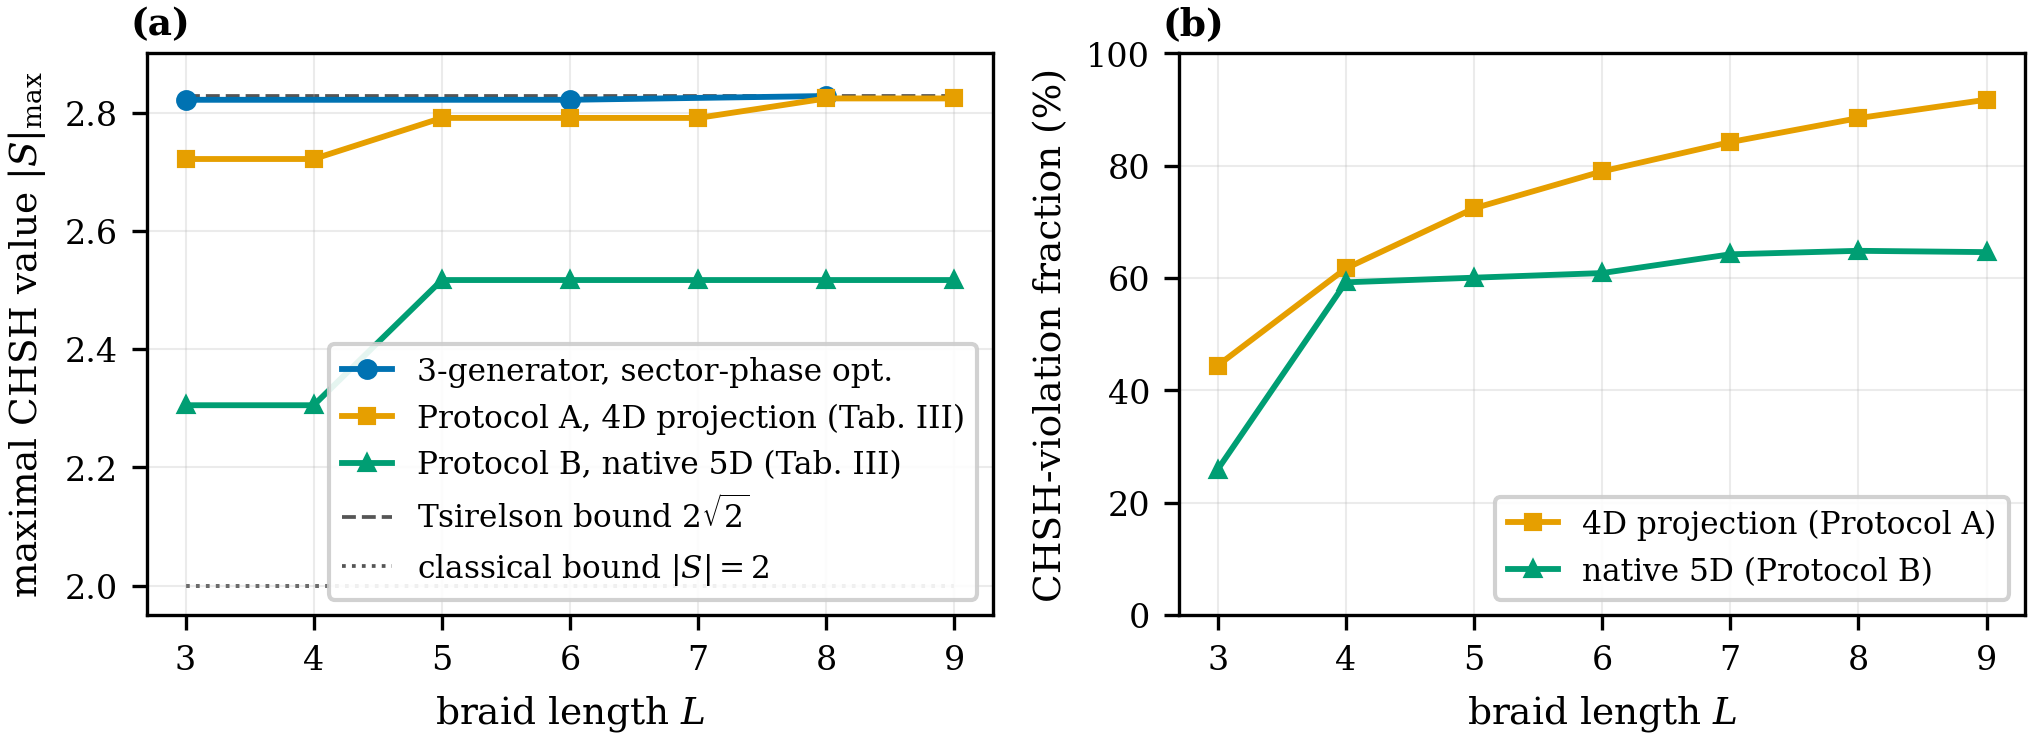
\includegraphics[width=0.9\textwidth]{figures/fig1_landscape.png}
\caption{\label{fig:landscape}%
Braiding-length dependence of the CHSH landscape.
(a)~Maximal CHSH value $|S|_{\max}$ versus braid length $L$ for the
three-generator encoding at the sector-phase optimum of the deposited
winning sequences (per-$L$ maxima of \texttt{s\_delta\_sweeps.json},
approaching the Tsirelson bound at $L=8$), and for
the two operational measurement protocols (Table~\ref{tab:protocol}):
Protocol~A (four-dimensional computational-subspace projection,
approaching $2\sqrt{2}$ within $0.16\%$) and Protocol~B (native
five-dimensional, trit-valued observables, saturating near $2.517$).
Dashed: Tsirelson bound $2\sqrt{2}$; dotted: classical bound $|S|=2$.
(b)~Fraction of braiding sequences with $|S|>2$ under the two
protocols, rising to $91.8\%$ (Protocol~A) and plateauing near
$64.6\%$ (Protocol~B) at $L=9$. Data: \texttt{landscape\_validation.json}
and \texttt{s\_delta\_sweeps.json}
(concept-DOI
10.5281/zenodo.19601352).}
\end{figure*}

Figure~\ref{fig:landscape} summarizes both protocols across braid
length. The two protocols agree qualitatively: under both, a majority of
braiding sequences violate the CHSH inequality for $L\geq 4$.
However, they differ quantitatively in two respects:

(i)~The maximal CHSH value in Protocol~B saturates at
$|S|^{5\text{D}}_{\max}\approx 2.517$ from $L=5$ onward,
while Protocol~A approaches the Tsirelson bound (within $0.16\%$).
The gap reflects the zero eigenvalue of the $X$ and $Y$ observables
on $|2\rangle$: a maximally entangled singlet-like state cannot be
fully realized in the five-dimensional space using trit-valued
observables.

(ii)~The CHSH fraction in Protocol~B plateaus near $64\text{--}65\%$,
compared to the monotonically rising fraction under Protocol~A.

\subsection{Leakage statistics}

The computational-subspace fidelity is the squared overlap onto the
orthonormal logical basis
$\{\ket{0},\ket{1},\ket{3},(\ket{2}+\ket{4})/\sqrt{2}\}$,
\begin{equation}
N^2 = |\psi_0|^2 + |\psi_1|^2 + |\psi_3|^2 + \tfrac{1}{2}|\psi_2+\psi_4|^2,
\end{equation}
which measures the fraction of the five-dimensional state that
survives projection into the two-qubit subspace and satisfies
$N^2\in[0,1]$ by construction.
At $L=9$, the minimum fidelity across all $19\,683$ sequences is
$N^2_{\min} = 0.131$, meaning that for some sequences up to $86.9\%$
of the amplitude resides outside the computational subspace.

This is consistent with the expectation that exact leakage-free
entangling gates may not exist for Fibonacci anyons~\cite{Cui2019}.
Protocol~A implicitly post-selects on the computational subspace by
renormalization; Protocol~B avoids this at the cost of a reduced
maximal $|S|$.

\subsection{Summary statement}

CHSH violation is generic under \emph{both} measurement protocols.
The qualitative finding---that a majority of Fibonacci braiding
sequences violate the CHSH inequality---is protocol-independent.
The quantitative CHSH fraction ($64.6\%$ vs.\ $91.8\%$ at $L=9$)
and the saturation value of $|S|_{\max}$ ($2.517$ vs.\ $2.824$)
are protocol-dependent, reflecting the incomplete flip symmetry
of the five-dimensional fusion space.

\textit{Note on terminology.}\, In this paper, ``Protocol~B'' refers
specifically to the bipartite native-$5$D CHSH evaluation with
trit-valued $Z$ and $X$-like observables on the full five-dimensional
fusion space (Sec.~\ref{sec:protocol}, this paper). Other companion
analyses that probe alternative nonbipartite CHSH constructions on
the same fusion space (e.g., minimal three-diagonal-parity
single-particle constructions) are distinct in scope and are not
covered by the present landscape; the bipartite Protocol~B used here
remains well-defined as a CHSH evaluation in its own right.

We emphasize that the $d_{1b}$ encoding
(Sec.~\ref{sec:reconciliation}, Table~\ref{tab:d1b}) operates
natively in four dimensions with no leakage and yields the
headline $|S|=2.811$ figure of the present landscape, the same
value adopted as the Fibonacci reference in
Ref.~\cite{Sayim2026topological}.

%% ====================================================================
%%  SECTION 6 — SEQUENTIAL BRAIDING
%% ====================================================================
\section{Sequential braiding and temporal correlations}
\label{sec:sequential}

We now complete the trio argument by demonstrating that sequential
braiding on a shared fusion space produces measurable temporal
correlations in the CHSH-value series.

\subsection{Setup}

A register of six Fibonacci anyons is initialized in the vacuum state
$|0\rangle$ and subjected to $N=1000$ sequential braiding steps.
At each step~$n$, a generator $g_n\in\{\sigma_2,\sigma_3,\sigma_4\}$
is drawn from a specified distribution, the state is updated as
$|\psi_n\rangle = g_n|\psi_{n-1}\rangle$, and its native
five-dimensional (Protocol~B, Sec.~\ref{sec:protocol}) CHSH value
$S_n = S[\psi_n]$ is recorded.
This is repeated for $M=20$ independent runs.

Three models are compared:

\emph{Model~A} (i.i.d.):
each generator is chosen uniformly at random ($p=1/3$ each).

\emph{Model~B} (Markov-persistent):
with probability $0.6$, the previous generator is repeated;
otherwise a uniform draw from the remaining two.

\emph{Model~C} (no $\sigma_3$):
generators drawn from $\{\sigma_2,\sigma_4\}$ only ($p=1/2$ each),
serving as a control.

\subsection{Pillar~2: Null test}

As a prerequisite, we verify that \emph{independent} sector phases
produce no autocorrelation.
Drawing $N=10\,000$ sector phases $\delta_i$
uniformly from $[0,2\pi]$ and computing the CHSH value for each,
the lag-1 autocorrelation is
$\text{ACF}(1) = +0.001$ (Model~A configuration) and
$\text{ACF}(1) = +0.010$ (d1b configuration),
both within the $95\%$ confidence interval
$\pm 1.96/\sqrt{N} = \pm 0.020$
(seeded evaluation deposited as
\texttt{d8\_acf\_null\_robustness.py}).

The null hypothesis (ACF~$=0$ under i.i.d.\ sectors) is not
rejected.
This confirms that any nonzero autocorrelation observed in the
sequential-braiding models is a genuine dynamical effect, not
a statistical artifact.

\subsection{Pillar~3: Sequential-braiding autocorrelation}

Table~\ref{tab:acf} presents the measured autocorrelation for the
three models.

\begin{table}[!htb]
\caption{%
Lag-1 autocorrelation of the CHSH time series under sequential
braiding.
Significance is measured against the shuffle confidence band
(1000 random permutations of the observed series).
}
\label{tab:acf}
\begin{ruledtabular}
\begin{tabular}{lcccc}
Model & Generators & ACF(1) & Significance & CHSH\% \\
\hline
A (i.i.d.) & $\sigma_2,\sigma_3,\sigma_4$ & $+0.343$ & $10.85\sigma$ & 99.2 \\
B (Markov) & $\sigma_2,\sigma_3,\sigma_4$ & $+0.361$ & $11.24\sigma$ & 98.6 \\
C (no $\sigma_3$) & $\sigma_2,\sigma_4$ & $0.000$ & $0.00\sigma$ & 0.0 \\
\end{tabular}
\end{ruledtabular}
\end{table}

Both Models~A and~B exhibit highly significant positive autocorrelation,
with Model~B only marginally above Model~A ($0.361$ vs.\ $0.343$).
This indicates that the autocorrelation arises primarily from
\emph{state continuity}---each braid step applies a finite rotation,
keeping $|\psi_n\rangle$ close to $|\psi_{n-1}\rangle$ in Hilbert
space---rather than from generator-level persistence.

Model~C produces identically zero autocorrelation, confirming
the $\sigma_3$-blocking result of Sec.~\ref{sec:switch} in a
time-resolved setting: without the cross-bipartition generator,
the CHSH series is constant at $|S|=2.000$ with zero variance.

The runs test reinforces the clustering structure: in Model~A,
only $1$ crossing of the $|S|=2$ threshold is observed per run,
compared to an i.i.d.\ expectation of approximately $16$.

\subsection{Robustness}

Replacing the vacuum initial state with a seeded random normalized
five-dimensional vector yields $\text{ACF}(1)=+0.318$ (Model~A) and
$+0.326$ (Model~B), confirming that the effect survives
initialization.

The full autocorrelation range across the four deposited setups
(vacuum and random initialization, Models A and B) is
$\text{ACF}(1)\in [0.31,\,0.37]$, with the representative value
for long runs (Model~A, vacuum start) being $+0.34$.

\subsection{The trio argument}

The three pillars combine to establish that the topological sector
structure is real, measurable, and not attributable to chance:

\emph{Pillar~1} (Sec.~\ref{sec:switch}): $\sigma_3$-blocking shows
that a single generator switches entanglement on and off---topology
controls access.

\emph{Pillar~2} (this section): the null test confirms that
i.i.d.\ sector phases produce no autocorrelation---the method has
no intrinsic bias.

\emph{Pillar~3} (this section): sequential braiding produces
$\text{ACF}(1)=+0.34$ at $>10\sigma$---the sector structure
generates genuine temporal correlations without additional
assumptions.

\subsection{Falsifiable prediction}

In an experiment with sequential anyon braiding, the detection
sequence of CHSH-violation outcomes should exhibit positive
autocorrelation. We define the signed per-run CHSH term
\begin{equation}
g_n = (-1)^{a_n b_n}\, x_n y_n \in \{-1,+1\},
\end{equation}
where $a_n,b_n\in\{0,1\}$ label the measurement settings and
$x_n,y_n\in\{-1,+1\}$ the outcomes of run $n$; $\text{ACF}(1)$ denotes
the lag-1 autocorrelation of the $g_n$ series.
Standard quantum mechanics---under the assumption of independent
measurement choices between runs---predicts no systematic positive
ACF beyond statistical fluctuations.
The specific value ($\text{ACF}(1)\approx 0.34$) is
model-dependent, but the qualitative prediction $\text{ACF}>0$ is a
signature specific to \emph{sequential} braiding on a shared fusion
register, distinct from the spacelike-separated, independently
re-prepared trials of loophole-free Bell-test data such as those of
Refs.~\cite{Hensen2015,Giustina2015,Shalm2015}.

As a null control, we computed $\text{ACF}(1)$ on the published
outcome sequence of the openly available loophole-free test of Hensen
\emph{et al.}~\cite{Hensen2015} (data DOI
10.4121/uuid:6e19e9b2-4a2d-40b5-8dd3-a660bf3c0a31, $N=245$ valid
trials), finding
$\text{ACF}(1)=-0.047$ ($-0.64\sigma$, $|\text{ACF}(1)|<0.125$ at
$2\sigma$)---consistent with zero, as expected: the sequential-braiding
mechanism proposed here is structurally absent from independently
re-prepared Bell trials, so this is a genuine null control rather
than a failed prediction. The earlier test of Giustina \emph{et
al.}~\cite{Giustina2015} is closed as a venue for this analysis, as
its outcome sequence is available only on request; the higher-statistics
Shalm--NIST test~\cite{Shalm2015}, although also openly available, was
not analyzed here.
The appropriate venue to test the sequential-braiding prediction is
a platform that physically implements braiding sequentially on a
shared register, such as the digital Fibonacci-anyon realization of
Xu \emph{et al.}~\cite{XuEtAl2024} or the digital non-Abelian
Ising-anyon braiding of Andersen \emph{et al.}~\cite{Google2023};
both are gate-based (digital) realizations rather than the analog
continuous-braiding transport assumed in the present model, a
distinction relevant to any quantitative comparison.
The memory loophole in sequential Bell-type
data is well
characterized~\cite{BarrettCollinsHardyKentPopescu2002}; related but
distinct analyses of the same loophole-free data sets include a
no-signaling test~\cite{AdenierKhrennikov2017} and a
Kolmogorov-complexity analysis of the outcome
sequences~\cite{KovalskyHniloAguero2018,KovalskyHniloAguero2018b},
neither of which computes the lag-1 ACF proposed here; improved
statistical methodology for Bell-experiment data is discussed in
Ref.~\cite{Gill2022}.

%% ====================================================================
%%  SECTION 7 — DISCUSSION
%% ====================================================================
\section{Discussion}
\label{sec:discussion}

\subsection{CHSH violation is generic}

The central finding of this work is that CHSH violation is not a
fine-tuned property of special braiding sequences but a generic
feature of the Fibonacci anyon landscape.
Under both measurement protocols, more than half of all braiding
sequences violate the CHSH inequality for braid lengths $L\geq 4$.
The optimal sequences exhibit palindromic structure in both encodings,
and the three-generator necessity (with two generators: $C=0$ always)
provides a clean algebraic explanation for why entanglement requires
topological connectivity across the bipartition.

\subsection{Topology as gatekeeper}

The $\sigma_3$-blocking result and the sequential-braiding
autocorrelation together establish a picture in which topology
does not create or destroy entanglement, but \emph{gates} it:
the topological pathway governs whether entanglement is
accessible through the available braiding operations.
This complements the mutual-information study of
Ref.~\cite{Sayim2026topological}, where topological sector labels
were found to correlate with Bell-type observables in finite lattice
models (there reported as a finite-size effect).

\subsection{Implications for topological quantum computation}

The $\sigma_3$-blocking mechanism has a direct interpretation in
the context of topological quantum computing:
any braiding protocol that inadvertently excludes the
cross-bipartition generator will produce zero entanglement,
regardless of circuit depth.
The leakage analysis (Sec.~\ref{sec:protocol}) shows that this
concern extends beyond gate selection to the measurement
protocol, as up to $86.9\%$ of state weight can reside outside
the computational subspace.
This reinforces the finding of Cui \emph{et al.}~\cite{Cui2019}
that exact leakage-free entangling gates for Fibonacci anyons
may not exist.

\subsection{Limitations}

Several limitations qualify our results:

(i)~All computations are \emph{numerical simulations} within the
idealized Fibonacci TQFT at zero temperature and zero decoherence.
The charge-parity correlator underlying the CHSH violation is
topologically robust against braiding-phase noise
(dephasing)~\cite{Nayak2008}: for a closed-form two-parameter
degradation model $|S| = 2\lambda^2\sqrt{1+v^4 C^2}$ (charge-survival
probability $\lambda$, dephasing visibility $v$, ideal concurrence
$C$), pure dephasing ($v<1$, $\lambda=1$) bounds $|S|$ from below by
the classical value 2 (attained only in the fully-dephased limit
$v\to0$) and never drives it below---the violation \emph{vanishes}
rather than surviving degraded. Only charge-changing quasiparticle poisoning ($\lambda<1$)
can push $|S|$ below~2, at the Werner-state
threshold~\cite{Horodecki1995} $\lambda^\ast=2^{-1/4}=0.8409$ for an
ideal ($C=1$) Bell state and $\lambda^\ast=0.8416$ for the actually
braided state ($C=0.9968$)---a poisoning tolerance of order $16\%$
per qubit before the classical bound is restored; this follows
directly from the Horodecki and Werner criteria and is not a new
bound. A gap-scaling trade-off follows: the thermal quasiparticle
poisoning rate is exponentially suppressed by the topological
gap~\cite{KarzigColePikulin2021} (Arrhenius factor
$e^{-\Delta/k_BT}$), so the universal $\nu=12/5$
Fibonacci candidate---with a measured activation gap of order tens
of mK~\cite{Zhang2012}, the smallest of the accessible platforms---is
the thermally most fragile of the
accessible non-Abelian platforms,
while the $\nu=5/2$ Ising gap is comparatively robust but not
computationally universal. A nonequilibrium quasiparticle floor can
exceed the equilibrium poisoning rate by orders of magnitude in
realistic samples and is decoupled from temperature, so the
limitation is not purely thermal and does not vanish as $T\to 0$.
The idealized $k=3$ Read--Rezayi identification of $\nu=12/5$ is
itself optimistic in one respect (particle-hole conjugation and
Landau-level mixing strengthen the effective
gap~\cite{Mong2017}) and pessimistic in another (companion anyons at
nearby fillings, observed in the first excited Landau
level~\cite{Pan2008}, add poisoning channels). We do not
quote a specific operation-time bound: non-Abelian braiding at
$\nu=12/5$ has not been experimentally demonstrated, so any
timescale estimate would be conditional on an identification---
$\nu=12/5$ as the Fibonacci-anyon $k=3$ Read--Rezayi
state---that is numerically supported but not experimentally
confirmed~\cite{Mong2017,Zhu2015,Pakrouski2016}. Measurement
imperfections beyond this poisoning model are not addressed here.

(ii)~The sector phase $\delta$ entering via
$R_\tau\to R_\tau\cdot e^{i\delta}$ parameterizes a family of
braid representations but is not derived from a first-principles
Chern-Simons path integral.

(iii)~The CHSH-violation fraction is protocol-dependent
(Sec.~\ref{sec:protocol}): $64.6\%$ and $91.8\%$ represent
different---both legitimate---definitions of measurement on the
fusion space.

(iv)~The autocorrelation prediction (Sec.~\ref{sec:sequential}) is
quantitatively setup-dependent ($\text{ACF}(1)\in [0.31,0.37]$
across the four deposited setups),
though qualitatively robust ($\text{ACF}>0$).

(v)~The $S(\delta)$ functional form becomes increasingly complex
at longer braid lengths: a six-term Fourier fit achieves
$R^2=0.997$ at $L=3$ but only $R^2=0.38$ at $L=12$ in the
five-dimensional encoding, indicating that the CHSH landscape
develops structure beyond simple harmonic description.

\subsection{Comparison with the independent fusion-sector construction of Xu, Ye, and You}
\label{sec:xuyeyou_comparison}

Independently and contemporaneously, Xu, Ye, and You~\cite{Xu2025}
have studied CHSH correlations on triplets of the Fibonacci-anyon
state $|\tau,\tau;1\rangle$ using a graded three-dimensional
fusion-sector Hilbert space $\mathcal{H}_1 \oplus \mathcal{H}_\tau$
with measurement operators of the form $A_\alpha = \operatorname{diag}(1,
[[\cos\alpha,\sin\alpha],[\sin\alpha,-\cos\alpha]])$ (their Eq.~(9)).
Their construction reaches
$|S|_{\max} = (4\sqrt{2}\varphi + 2)/\varphi^3 \approx 2.633$
with superactivation as the underlying phenomenon: a single copy of
$|\tau,\tau;1\rangle$ admits a local hidden-variable model, while three
copies activate Bell nonlocality. Their setup is bipartite under the
graded tensor product, with $A_\alpha$ block-diagonal across
$\mathcal{H}_1$ and $\mathcal{H}_\tau$. Tsirelson's bound $2\sqrt{2}$
applies in their setting; the value $2.633$ is sub-Tsirelson due to
nonuniform Schmidt weights of the three-copy state
(weight $2/\varphi^2 \approx 0.764$ on $\mathcal{H}_\tau \otimes \mathcal{H}_\tau$).

The present paper's $d_{1b}$ four-dimensional encoding, by contrast,
operates on a single copy of an entangled four-dimensional fusion
state with concurrence $C = 0.988$, reaching $|S| = 2.811$ at
$\delta/\pi = 1.76$, which saturates the bipartite Horodecki bound
$2\sqrt{1+C^2}$ for this concurrence. The two constructions address
different questions (multi-copy activation versus single-copy braid-
induced violation) and produce different but compatible values:
both respect Tsirelson's bound, both bipartite Bell-operator norms
equal $2\sqrt{2}$ exactly, and the difference reflects distinct
Schmidt structures of the underlying states. An independent
reproduction of both values, together with the
$|S| = 3.406$ value from the companion
paper~\cite{Sayim2026chsh} (which uses a nonbipartite
construction violating setting-locality, not subject to Tsirelson's
bound), is documented in
a dedicated comparison analysis of the project
repository: all three values are reproduced to within their natural
precisions, Bell-operator-norm comparisons confirm the structural
distinction, and the standard sanity tests (state norm,
outcome-probability summation, operator-norm vs algebraic bound)
exclude post-selection or nonstandard normalization in any of the
three constructions.

\subsection{Outlook}

The present enumeration is bounded at $L=12$ by the $3^L$ scaling;
other anyon models (Ising, $\text{SU}(2)_k$ for $k>3$) and experimental
autocorrelation data are not addressed here.
Whether the Kitaev honeycomb model~\cite{Kitaev2006}, which offers a
lattice setting in which both classical and quantum limits are accessible,
can bridge the present work with the $\mathbb{Z}_2$ results of
Ref.~\cite{Sayim2026topological} remains an open question.
A further open question, suggested by the Schmidt-rank-3 structure
of the Xu, Ye, You construction~\cite{Xu2025}, is whether a
single-copy Schmidt-rank-3 state in the four-dimensional $d_{1b}$
Hilbert space (or in the five-dimensional fusion space) could be
prepared by a different braiding protocol; whether such a state would
yield CHSH values intermediate between the present results remains open.

%% ====================================================================
%%  CONCLUSION
%% ====================================================================
\section{Conclusion}
\label{sec:conclusion}

We have presented the first, to our knowledge, complete sequence-by-sequence enumeration of CHSH
violation across all Fibonacci anyon braiding words of length $L=3$--$12$ in
two complementary encodings, in the broader landscape of qualitative
Bell-test constructions on Fibonacci/Ising and Majorana
platforms~\cite{Brennen2009,ChangChuMa2017,Drummond2014,RomitoGefen2017,ClarkeSauDasSarma2016}
and the independently and contemporaneously analyzed three-copy fusion-sector
construction of Xu, Ye, and You~\cite{Xu2025}; a companion
Leggett--Garg-inequality letter on the same Fibonacci representation,
saturating the L\"uders bound $K_3 \to 3/2$, is reported
in Ref.~\cite{Sayim2026LGI}.

CHSH violation is generic: $64.6\%$ of sequences violate the CHSH
inequality under native five-dimensional measurement, and $91.8\%$
under computational-subspace projection, at $L=9$.

The optimal $d_{1b}$ sequence at $L=12$ reaches $|S|=2.811$
($99.4\%$ of the Tsirelson bound $2\sqrt{2}$, $C=0.988$), while the
three-generator encoding on the full five-dimensional fusion space
approaches the Tsirelson bound ($|S|=2.824$, $99.84\%$) already at
$L=8$.

Topology acts as a gatekeeper through the $\sigma_3$ switch:
removing the cross-bipartition generator collapses entanglement
to zero exactly, independent of sequence length, sector phase,
and encoding.

Sequential braiding on a shared anyon register produces positive
lag-1 autocorrelation ($\text{ACF}(1)=+0.34$ at $10.85\sigma$),
a falsifiable signature of state continuity that, under the assumption
of independent measurement settings between runs, is not predicted by
standard quantum mechanics.

We emphasize that the CHSH values reported here, while in excess of the
classical bound, should not be interpreted as Bell violations in
the EPR sense (cf.\ Sec.~\ref{fn:nonsep}): the underlying Fibonacci
fusion space does not factorize as a tensor product of local Alice and
Bob subsystems, and the classical-bound excess is more precisely
characterized as a signature of topological nonseparability in
fusion space.

Together with the finite-size mutual-information correlations
reported in Ref.~\cite{Sayim2026topological}, these findings indicate
that the available topological operations gate whether CHSH
correlations are accessible---a structural pattern seen, with the
caveats noted there, in finite classical lattice systems and in
quantum anyon systems alike.

%% ====================================================================
%%  DATA AND CODE AVAILABILITY
%% ====================================================================
\section*{Data and Code Availability}

The deterministic scripts and JSON output files that validate the
results reported in this paper are archived on Zenodo under the
concept DOI
\href{https://doi.org/10.5281/zenodo.19601352}{10.5281/zenodo.19601352}
(which always resolves to the latest version) and released under the
Creative Commons Attribution 4.0 International (CC BY 4.0) license.
The archive includes the three-generator (5D) landscape validation
and its leakage-norm reanchor (\texttt{landscape\_validation.py},
\texttt{n2\_reanchor.py}); a closed-form sector-phase sweep validation
covering all rows of Table~\ref{tab:d1b} and the sequences of
Table~\ref{tab:3gen}
(\texttt{d4\_s\_delta\_sweep\_validation.py}, reproducing
\texttt{s\_delta\_sweeps.json} and the printed table values); the topological-gatekeeper validation,
including the exact $\sigma_3$-block $C=0$ check
(\texttt{d5\_topology\_switch\_validation.py}, reproducing
\texttt{topology\_switch\_results.json}); the sequential-braiding
autocorrelation prediction of Table~\ref{tab:acf}
(\texttt{d6\_acf\_prediction\_sequential\_braiding.py}); the seeded
Pillar-2 null test and initialization-robustness evaluation of
Sec.~\ref{sec:sequential}
(\texttt{d8\_acf\_null\_robustness.py}); and an
independent null-control reanalysis of the Hensen \emph{et al.}\
(2015) loophole-free Bell data, including the underlying public
dataset (\texttt{d7\_acf\_hensen2015\_null\_control.py}). The
exhaustive sequence search that originally identified the winning
braid words reported in Tables~\ref{tab:d1b} and~\ref{tab:3gen}, and
the verification scripts for the sector-phase Yang--Baxter check of
Appendix~\ref{app:algebra} (Table~\ref{tab:yb_under_delta}), are not
part of this record.

%% ====================================================================
%%  USE OF AI TOOLS
%% ====================================================================
\section*{Use of AI tools}

In the research, processing, and writing of this paper and its results I worked together with generative AI tools, in practice a system of multiple coordinated AI instances that I set up and orchestrate (large language models, mainly Claude, by Anthropic, inside Claude Code). At their current context sizes I found it far more effective to work with several specialized instances, each with its own role and its own harness of rules and parameters that I designed and refined through feedback, than to load a single instance with all of the material; for my workflow that would have been inefficient, though this depends on the individual implementation. I lead this collaboration: I choose the research directions, set the goals, and make the final decisions in open exchange with the AI, learning actively as the work proceeds. The AI carries out the drafting, including the mathematical and technical parts, the numerical computation, and the literature search, under my direction. The AI works autonomously only task by task, within the structure I develop through feedback: it completes a task, and at open questions that need me it stops until the point is settled before the next step. Along the way I witness and take many of the decisions that shape the path, and it is common for me to spot things that need improvement. The work spans many separate runs, and a single simulation or build task alone can take up to an hour, so it could not happen all together in one autonomous run; and had I let the AI do all of it together alone, even if it is possible, it would no longer be my work but the AI's.

I run multiple verifications at the different stages of the work and one before release, including cross-checks with an unrelated AI model from a different company, and all references are checked against the original sources. In the end what matters are human eyes, a principle that is itself written into the parameters of my system: I reach out to experts after publishing for review and feedback, so I learn what is solid and what must be corrected or falsified. My scripts for reproduction and review are released with this record. These tools are not authors; I am the author, and I take full responsibility for all scientific content and decisions leading to these results and their publication.

%% ====================================================================
%%  ACKNOWLEDGMENTS
%% ====================================================================
\begin{acknowledgments}
This research received no specific grant from any funding agency in the
public, commercial, or not-for-profit sectors. The author declares no
competing interests.
\end{acknowledgments}

%% ====================================================================
%%  APPENDIX
%% ====================================================================
\appendix

\section{Braid-generator matrices}
\label{app:generators}

The five braid generators $\sigma_1,\ldots,\sigma_5$ for six
Fibonacci anyons in the basis~\eqref{eq:basis} are constructed
as follows.
For each generator $\sigma_k$, the anyon pair $(\tau_k,\tau_{k+1})$
is braided via the $F$-move/R-phase/$F$-move sequence on the
relevant two-dimensional subspace of the fusion tree.
The remaining basis states acquire diagonal $R$-phases.
Explicit $5\times 5$ matrices are provided in the supplementary
code archived with the Zenodo deposit.

The key structural properties:
\begin{itemize}
\item $\sigma_2$ mixes states within the $x_1\in\{1,\tau\}$
subspace (Alice's qubit), preserving $x_3$.
\item $\sigma_4$ mixes states within the $x_3\in\{1,\tau\}$
subspace (Bob's qubit), preserving $x_1$.
\item $\sigma_3$ re-fuses the intermediate label $x_2$, coupling
both branches of the fusion tree.
\item $\sigma_1$ and $\sigma_5$ act as diagonal phases on $x_1$
and $x_3$ respectively.
\end{itemize}

\section{Fourier structure of $S(\delta)$}
\label{app:fourier}

The CHSH value as a function of sector phase $\delta$ exhibits
encoding-dependent harmonic structure.
For the Ising anyon model, the functional form is exactly
$S(\delta) = 2\sqrt{2}\cos^2(\delta/2)$, containing only the
fundamental harmonic $n=1$. This idealized Ising result assumes
access to a nonstabilizer (``magic'') single-qubit operation beyond
the topologically protected Clifford gate set; purely stabilizer
operations on Ising anyons cannot violate the CHSH
inequality~\cite{HowardVala2012}.
For Fibonacci anyons, the leading nonconstant harmonic of a
six-term Fourier fit at $L=3$ ($\sigma_4\sigma_2\sigma_3$ sequence,
$R^2=0.997$) is $n=4$:
\begin{align}
S(\delta) \approx{} &1.931 - 0.040\cos\delta + 0.126\sin\delta
\nonumber \\
&+ 0.293\cos 2\delta + 0.212\sin 2\delta \nonumber \\
&- 0.098\cos 3\delta + 0.072\sin 3\delta \nonumber \\
&+ 0.141\cos 4\delta + 0.430\sin 4\delta \nonumber \\
&+ 0.025\cos 5\delta.
\label{eq:fourier}
\end{align}
The apparent spectral contrast between Fibonacci (leading harmonic
$n=4$ in this fit) and Ising (exactly $n=1$) is suggestive of
order-dependent CHSH signatures, but the dominant-harmonic
assignment is sensitive to the fit method and the sector-phase
sampling (cf.\ the low fit quality at larger $L$ below) and we do
not pin it as a sharp invariant.

At longer braid lengths, $R^2$ decreases ($R^2=0.38$ at $L=12$
in the 5D encoding), indicating that the $S(\delta)$ landscape
develops structure beyond six-term Fourier description.

\section{Verification of the five-dimensional representation under sector-phase modulation}
\label{app:algebra}

The qualitative nonseparability and contextuality framing of Sec.~\ref{fn:nonsep} and
Sec.~\ref{sec:encodings} is supported by an independent numerical check
of the braid-group relations for the full five-state generators
$\sigma_1, \ldots, \sigma_5$ across a range of sector phases $\delta$.
At $\delta = 0$ the standard Fibonacci modular tensor category is
satisfied to floating-point precision (Yang--Baxter residuum
$\leq 8.2 \times 10^{-16}$, distant commutators identically zero).
Under the sector-phase modulation
$R_\tau \mapsto R_\tau \cdot e^{i\delta}$ introduced in
Sec.~\ref{sec:encodings} to parameterize the family of
representations on the torus, Yang--Baxter deforms uniformly across
all four neighboring generator pairs while distant commutators
$[\sigma_i, \sigma_j] = 0$ for $|i-j| \geq 2$ remain identically zero
throughout. Table~\ref{tab:yb_under_delta} summarizes the verification.
The sector phase $\delta$ is thus a free deformation knob rather than a
physical parameter: generic $\delta \neq 0$ breaks the Yang--Baxter/hexagon
consistency of the representation (Table~\ref{tab:yb_under_delta}), and only
$\delta = 0$ recovers the standard Fibonacci modular tensor category. This
expected discreteness --- rather than a continuum of consistent deformations
--- is consistent with the general Ocneanu-rigidity result for fusion
categories~\cite{EtingofNikshychOstrik2002}, which here rests on the
paper-internal numerics of Table~\ref{tab:yb_under_delta} rather than on an
independent categorical classification of this specific representation.

\begin{table}[h]
\caption{Algebraic verification of the five-state representation under
sector-phase modulation. The Yang--Baxter residuum
$\|\sigma_i\sigma_{i+1}\sigma_i - \sigma_{i+1}\sigma_i\sigma_{i+1}\|_F$
is identical across all four neighboring pairs and is shown in column 2.
The distant commutator $\|[\sigma_i, \sigma_j]\|_F$ for $|i-j| \geq 2$
is zero to all available numerical precision (exact, not float-floor) for
every tested $\delta$.}
\label{tab:yb_under_delta}
\begin{ruledtabular}
\begin{tabular}{rcc}
$\delta/\pi$ & YB residuum (5D) & distant commutator (5D) \\
\hline
$0.000$ & $\leq 8.2 \times 10^{-16}$ & $0$ (exact) \\
$0.100$ & $0.525$ & $0$ (exact) \\
$0.250$ & $0.958$ & $0$ (exact) \\
$0.500$ & $0.473$ & $0$ (exact) \\
$1.000$ & $0.873$ & $0$ (exact) \\
$1.191$ & $0.052$ & $0$ (exact) \\
$1.500$ & $1.523$ & $0$ (exact) \\
\end{tabular}
\end{ruledtabular}
\end{table}

The intact $\delta = 0$ representation confirms that the
failure of tensor-product factorization underlying the $d_{1b}$ encoding
(Sec.~\ref{sec:encodings}, Sec.~\ref{fn:nonsep}) is a property of
the deliberate four-dimensional projection of the
five-dimensional fusion space, not of the underlying braid
representation itself. The exact preservation of distant commutativity
under $\delta$-modulation is structural: the modulation acts locally
on the $R_\tau$ eigenvalue and does not couple block- or
diagonally-separated generators. The companion Leggett--Garg
analysis~\cite{Sayim2026LGI} reports an analogous fixed-word vs
envelope distinction for the temporal $K_3(\delta)$ periodicity.
All values above were verified with the deterministic scripts
\texttt{d2\_delta\_phase\_consistency.py} and
\texttt{d3\_5d\_braid\_algebra\_consistency.py}, which document the
full underlying data including the $\mathbb{Z}_5$ phase spectrum of
$\Delta^2$ from the Birman formula and the $d_{1b}$ spectator-filter
algebra-breaks; these two scripts are not part of this record.

%% ====================================================================
%%  REFERENCES
%% ====================================================================

\begin{thebibliography}{44}

\bibitem{Sayim2026topological}
B.~Y.~Sayim,
\textit{Sector-Dependent CHSH Violation in Fibonacci Anyons,
and Finite-Size Topological--CHSH Mutual Information in 2D
Lattice Models},
Zenodo preprint (2026),
\href{https://doi.org/10.5281/zenodo.19600752}{doi:10.5281/zenodo.19600752}.

\bibitem{Sayim2026chsh}
B.~Y.~Sayim,
\textit{CHSH-Form Values Without Bell Nonlocality: Inapplicability of the
Tsirelson Bound on a Non-Factorized Fibonacci Fusion Space},
Zenodo preprint (2026),
\href{https://doi.org/10.5281/zenodo.19601998}{doi:10.5281/zenodo.19601998}.

\bibitem{Nayak2008}
C.~Nayak, S.~H.~Simon, A.~Stern, M.~Freedman, and S.~Das~Sarma,
\textit{Non-Abelian anyons and topological quantum computation},
Rev.\ Mod.\ Phys.\ \textbf{80}, 1083 (2008).

\bibitem{Freedman2003}
M.~H.~Freedman, A.~Kitaev, M.~J.~Larsen, and Z.~Wang,
\textit{Topological quantum computation},
Bull.\ Am.\ Math.\ Soc.\ \textbf{40}, 31 (2003).

\bibitem{Bonesteel2005}
N.~E.~Bonesteel, L.~Hormozi, G.~Zikos, and S.~H.~Simon,
\textit{Braid topologies for quantum computation},
Phys.\ Rev.\ Lett.\ \textbf{95}, 140503 (2005).

\bibitem{Hormozi2007}
L.~Hormozi, G.~Zikos, N.~E.~Bonesteel, and S.~H.~Simon,
\textit{Topological quantum compiling},
Phys.\ Rev.\ B \textbf{75}, 165310 (2007).

\bibitem{Horodecki1995}
R.~Horodecki, P.~Horodecki, and M.~Horodecki,
\textit{Violating Bell inequality by mixed spin-$\frac{1}{2}$
states: necessary and sufficient condition},
Phys.\ Lett.\ A \textbf{200}, 340 (1995).

\bibitem{Cui2019}
S.~X.~Cui, K.~T.~Tian, J.~F.~Vasquez, Z.~Wang, and H.~M.~Wong,
\textit{The search for leakage-free entangling Fibonacci braiding gates},
J.\ Phys.\ A: Math.\ Theor.\ \textbf{52}, 455301 (2019);
\href{https://arxiv.org/abs/1904.01731}{arXiv:1904.01731}.

\bibitem{Burke2024}
P.~C.~Burke, C.~Aravanis, J.~Aspman, J.~Mare\v{c}ek, and J.~Vala,
\textit{Topological quantum compilation of two-qubit gates},
arXiv:2408.07132 (2024).

\bibitem{Yang2019}
Z.-C.~Yang, K.~Meichanetzidis, S.~Kourtis, and C.~Chamon,
\textit{Scrambling via braiding of nonabelions},
Phys.\ Rev.\ B \textbf{99}, 045132 (2019).

\bibitem{Google2023}
T.~I.~Andersen \emph{et al.} (Google Quantum AI),
\textit{Non-Abelian braiding of graph vertices in a
superconducting processor},
Nature \textbf{618}, 264 (2023);
\href{https://arxiv.org/abs/2210.10255}{arXiv:2210.10255}.


\bibitem{Hensen2015}
B.~Hensen \emph{et al.},
\textit{Loophole-free Bell inequality violation using electron
spins separated by 1.3 kilometres},
Nature \textbf{526}, 682 (2015).

\bibitem{Giustina2015}
M.~Giustina \emph{et al.},
\textit{Significant-loophole-free test of Bell's theorem with
entangled photons},
Phys.\ Rev.\ Lett.\ \textbf{115}, 250401 (2015).


\bibitem{Kitaev2006}
A.~Kitaev,
\textit{Anyons in an exactly solved model and beyond},
Ann.\ Phys.\ \textbf{321}, 2 (2006).



\bibitem{Brennen2009}
G.~K.~Brennen, S.~Iblisdir, J.~K.~Pachos, and J.~K.~Slingerland,
\textit{Non-locality of non-Abelian anyons},
New J.\ Phys.\ \textbf{11}, 103023 (2009);
\href{https://arxiv.org/abs/0810.4319}{arXiv:0810.4319}.

\bibitem{ChangChuMa2017}
P.-Y.~Chang, S.-K.~Chu, and C.-T.~Ma,
\textit{Bell's inequality and entanglement in qubits},
J.\ High Energy Phys.\ \textbf{09} (2017) 100;
\href{https://arxiv.org/abs/1705.06444}{arXiv:1705.06444}.

\bibitem{Drummond2014}
D.~E.~Drummond, A.~A.~Kovalev, C.-Y.~Hou, K.~Shtengel, and L.~P.~Pryadko,
\textit{Demonstrating entanglement by testing Bell's theorem in Majorana wires},
Phys.\ Rev.\ B \textbf{90}, 115404 (2014);
\href{https://arxiv.org/abs/1403.0916}{arXiv:1403.0916}.

\bibitem{RomitoGefen2017}
A.~Romito and Y.~Gefen,
\textit{Ubiquitous nonlocal entanglement with Majorana zero modes},
Phys.\ Rev.\ Lett.\ \textbf{119}, 157702 (2017);
\href{https://arxiv.org/abs/1703.01841}{arXiv:1703.01841}.

\bibitem{ClarkeSauDasSarma2016}
D.~J.~Clarke, J.~D.~Sau, and S.~Das~Sarma,
\textit{A practical phase gate for producing Bell violations in Majorana wires},
Phys.\ Rev.\ X \textbf{6}, 021005 (2016);
\href{https://arxiv.org/abs/1510.00007}{arXiv:1510.00007}.

\bibitem{Xu2025}
C.-Q.~Xu, W.~Ye, and L.~You,
\textit{Superactivation of Bell nonlocality in pure anyonic states},
Phys.\ Rev.\ A \textbf{112}, 062232 (2025);
\href{https://arxiv.org/abs/2506.08919}{arXiv:2506.08919}.

\bibitem{Sorella2023}
S.~P.~Sorella,
\textit{On the representations of Bell's operators in Quantum Mechanics},
Found.\ Phys.\ \textbf{53}, 59 (2023);
\href{https://arxiv.org/abs/2304.05696}{arXiv:2304.05696}.

\bibitem{Sayim2026LGI}
B.~Y.~Sayim,
\textit{Leggett--Garg saturation and structural signatures in Fibonacci-anyon braiding},
Zenodo preprint (2026),
\href{https://doi.org/10.5281/zenodo.20372744}{doi:10.5281/zenodo.20372744}.


\bibitem{GuimaraesRoditiSorella2024}
M.~S.~Guimaraes, I.~Roditi, and S.~P.~Sorella,
\textit{Bell-CHSH inequality and unitary operators},
Nucl.\ Phys.\ B (2024);
\href{https://arxiv.org/abs/2403.15276}{arXiv:2403.15276}.

\bibitem{Chou2025}
T.-M.~Chou,
\textit{Topological Contextuality and Quantum Representations},
\href{https://arxiv.org/abs/2506.14537}{arXiv:2506.14537} (2025).

\bibitem{BondersonKnappPatel2017}
P.~Bonderson, C.~Knapp, and K.~Patel,
\textit{Anyonic Entanglement and Topological Entanglement Entropy},
\href{https://arxiv.org/abs/1706.09420}{arXiv:1706.09420} (2017).

\bibitem{EtingofNikshychOstrik2002}
P.~Etingof, D.~Nikshych, and V.~Ostrik,
\textit{On fusion categories},
\href{https://arxiv.org/abs/math/0203060}{arXiv:math/0203060} (2002).

\bibitem{KarzigColePikulin2021}
T.~Karzig, W.~S.~Cole, and D.~I.~Pikulin,
\textit{Quasiparticle Poisoning of Majorana Qubits},
Phys.\ Rev.\ Lett.\ \textbf{126}, 057702 (2021).

\bibitem{Mong2017}
R.~S.~K.~Mong, M.~P.~Zaletel, F.~Pollmann, and Z.~Papi\'{c},
\textit{Fibonacci anyons and charge density order in the 12/5 and 13/5 plateaus},
Phys.\ Rev.\ B \textbf{95}, 115136 (2017);
\href{https://arxiv.org/abs/1505.02843}{arXiv:1505.02843}.

\bibitem{Zhang2012}
C.~Zhang, C.~Huan, J.~S.~Xia, N.~S.~Sullivan, W.~Pan, K.~W.~Baldwin, K.~W.~West, L.~N.~Pfeiffer, and D.~C.~Tsui,
\textit{Spin Polarization of the 12/5 Fractional Quantum Hall Effect},
\href{https://arxiv.org/abs/1204.0560}{arXiv:1204.0560} (2012).

\bibitem{Pakrouski2016}
K.~Pakrouski, M.~Troyer, Y.-L.~Wu, S.~Das~Sarma, and M.~R.~Peterson,
\textit{The enigmatic 12/5 fractional quantum Hall effect},
Phys.\ Rev.\ B \textbf{94}, 075108 (2016);
\href{https://arxiv.org/abs/1604.04610}{arXiv:1604.04610}.

\bibitem{Zhu2015}
W.~Zhu, S.~S.~Gong, F.~D.~M.~Haldane, and D.~N.~Sheng,
\textit{The Fractional Quantum Hall States at $\nu=13/5$ and $12/5$ and their Non-Abelian Nature},
\href{https://arxiv.org/abs/1505.03050}{arXiv:1505.03050} (2015).

\bibitem{Pan2008}
W.~Pan, J.~S.~Xia, H.~L.~Stormer, D.~C.~Tsui, C.~Vicente, E.~D.~Adams, N.~S.~Sullivan, L.~N.~Pfeiffer, K.~W.~Baldwin, and K.~W.~West,
\textit{Experimental studies of the fractional quantum Hall effect in the first excited Landau level},
Phys.\ Rev.\ B \textbf{77}, 075307 (2008);
\href{https://arxiv.org/abs/0801.1318}{arXiv:0801.1318}.


\bibitem{Shalm2015}
L.~K.~Shalm \emph{et al.},
\textit{A strong loophole-free test of local realism},
Phys.\ Rev.\ Lett.\ \textbf{115}, 250402 (2015);
\href{https://arxiv.org/abs/1511.03189}{arXiv:1511.03189}.

\bibitem{BarrettCollinsHardyKentPopescu2002}
J.~Barrett, D.~Collins, L.~Hardy, A.~Kent, and S.~Popescu,
\textit{Quantum nonlocality, Bell inequalities and the memory loophole},
Phys.\ Rev.\ A \textbf{66}, 042111 (2002);
\href{https://arxiv.org/abs/quant-ph/0205016}{arXiv:quant-ph/0205016}.

\bibitem{AdenierKhrennikov2017}
G.~Adenier and A.~Yu.~Khrennikov,
\textit{Test of the no-signaling principle in the Hensen ``loophole-free CHSH experiment''},
Fortschr.\ Phys.\ \textbf{65}, 1600096 (2017);
\href{https://arxiv.org/abs/1606.00784}{arXiv:1606.00784}.

\bibitem{KovalskyHniloAguero2018}
M.~G.~Kovalsky, A.~A.~Hnilo, and M.~B.~Ag\"uero,
\textit{Kolmogorov complexity of sequences of random numbers generated in Bell's experiments},
Phys.\ Rev.\ A \textbf{98}, 042131 (2018);
\href{https://arxiv.org/abs/1805.07161}{arXiv:1805.07161}.

\bibitem{KovalskyHniloAguero2018b}
M.~G.~Kovalsky, A.~A.~Hnilo, and M.~B.~Ag\"uero,
\textit{Addendum to: Kolmogorov complexity of sequences of random numbers generated in Bell's experiments (series of outcomes)},
\href{https://arxiv.org/abs/1812.05926}{arXiv:1812.05926} (2018).

\bibitem{DeFabritiisEtAl2023}
P.~De~Fabritiis, F.~M.~Guedes, M.~S.~Guimaraes, G.~Peruzzo, I.~Roditi, and S.~P.~Sorella,
\textit{Weyl operators, Tomita--Takesaki theory, and Bell--Clauser-Horne-Shimony-Holt inequality violations},
Phys.\ Rev.\ D \textbf{108}, 085026 (2023);
\href{https://arxiv.org/abs/2309.02941}{arXiv:2309.02941}.

\bibitem{SummersWerner1987}
S.~J.~Summers and R.~F.~Werner,
\textit{Maximal violation of Bell's inequalities is generic in quantum field theory},
Commun.\ Math.\ Phys.\ \textbf{110}, 247 (1987).

\bibitem{JiNatarajanVidickWrightYuen2020}
Z.~Ji, A.~Natarajan, T.~Vidick, J.~Wright, and H.~Yuen,
\textit{MIP*=RE},
\href{https://arxiv.org/abs/2001.04383}{arXiv:2001.04383} (2020).

\bibitem{FanDeGaris2010}
Z.~Fan and H.~de~Garis,
\textit{Braid Matrices and Quantum Gates for Ising Anyons Topological Quantum Computation},
Eur.\ Phys.\ J.\ B \textbf{74}, 419 (2010);
\href{https://arxiv.org/abs/1003.1253}{arXiv:1003.1253}.

\bibitem{HowardVala2012}
M.~Howard and J.~Vala,
\textit{Nonlocality as a Benchmark for Universal Quantum Computation in Ising Anyon Topological Quantum Computers},
Phys.\ Rev.\ A \textbf{85}, 022304 (2012);
\href{https://arxiv.org/abs/1112.1516}{arXiv:1112.1516}.

\bibitem{XuEtAl2024}
S.~Xu \emph{et al.},
\textit{Non-Abelian braiding of Fibonacci anyons with a superconducting processor},
\href{https://arxiv.org/abs/2404.00091}{arXiv:2404.00091} (2024).

\bibitem{Gill2022}
R.~D.~Gill,
\textit{Optimal statistical analyses of Bell experiments},
\href{https://arxiv.org/abs/2209.00702}{arXiv:2209.00702} (2022).

\end{thebibliography}

\end{document}

